\begin{figure}[h]
\centering
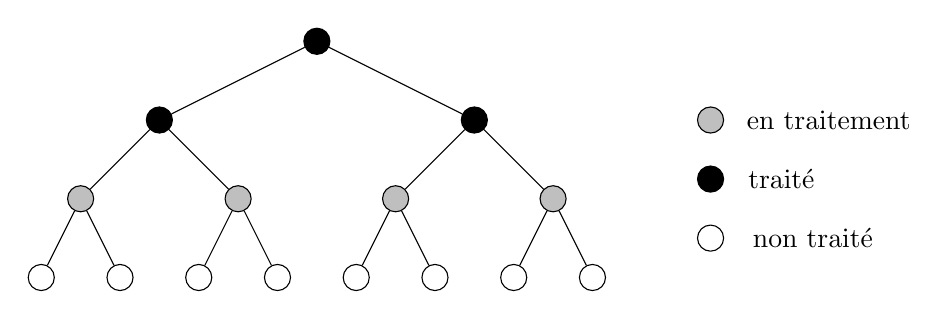
\begin{tikzpicture}
%%%%%%%%%%%%%%%%%%%%%%%%%%%%%%%%%%%%%%%%%%%%%%%%%%%%%%%%
% STYLE
\tikzstyle{processor}=[rectangle,draw]
\tikzstyle{b}=[circle,draw]
\tikzstyle{bc}=[circle,draw,fill=gray!50]
\tikzstyle{bt}=[circle,draw,fill=black]
\tikzstyle{txt}=[]

%%%%%%%%%%%%%%%%%%%%%%%%%%%%%%%%%%%%%%%%%%%%%%%%%%%%%%%%
% NODES
\node[bt] (N00) at (0,0) {};

\node[bt] (N10) at (-2,-1) {};
\node[bt] (N11) at (2,-1) {};

\node[bc] (N20) at (-3,-2) {};
\node[bc] (N21) at (3,-2) {};
\node[bc] (N22) at (-1,-2) {};
\node[bc] (N23) at (1,-2) {};

\node[b] (N30) at (-3.5,-3) {};
\node[b] (N31) at (3.5,-3) {};
\node[b] (N32) at (-1.5,-3) {};
\node[b] (N33) at (1.5,-3) {};
\node[b] (N34) at (-2.5,-3) {};
\node[b] (N35) at (2.5,-3) {};
\node[b] (N36) at (-0.5,-3) {};
\node[b] (N37) at (0.5,-3) {};

\node[bc] (L0) at (5,-1) {};
\node[bt] (L1) at (5,-1.75) {};
\node[b] (L2) at (5,-2.5) {};

\node[txt] (t5) at (6.5,-1) {en traitement};
\node[txt] (t6) at (5.9,-1.75) {traité};
\node[txt] (t7) at (6.3,-2.5) {non traité};
%%%%%%%%%%%%%%%%%%%%%%%%%%%%%%%%%%%%%%%%%%%%%%%%%%%%%%%%
% LINKS
\draw (N00) -- (N10);
\draw (N00) -- (N11);

\draw (N10) -- (N20);
\draw (N10) -- (N22);
\draw (N11) -- (N21);
\draw (N11) -- (N23);

\draw (N20) -- (N30);
\draw (N21) -- (N31);
\draw (N22) -- (N32);
\draw (N23) -- (N33);
\draw (N20) -- (N34);
\draw (N21) -- (N35);
\draw (N22) -- (N36);
\draw (N23) -- (N37);

\end{tikzpicture}
\caption*{Schématisation de \emph{blocage} des threads dans l'arbre de récursivité avec $4$ threads}
\end{figure}